%************************************************
\chapter{Bounding Mean First-Passage Times}\label{ch:MFPT}






%\title{Bounding Mean First Passage Times in\\   Population Continuous-Time
%Markov Chains}
%\titlerunning{Bounding Mean First Passage Times in \acp{MPM}}
%\author{Michael Backenk\"ohler${}^{1,2}$, Luca Bortolussi${}^{3,1}$, Verena Wolf${}^{1}$}
%\authorrunning{M.\ Backenk\"ohler et al.}
%\institute{${}^{1}$Saarland University, Germany,\\ ${}^{2}$ Saarbr\"ucken Graduate School of Computer Science,\\
%${}^{3}$University of Trieste, Italy}
%\maketitle
%\begin{abstract}
%  We consider the problem of bounding mean first passage times and reachability probabilities
%  for the class of population continuous-time Markov chains,  which capture stochastic interactions between groups of identical agents.
%  The  quantitative analysis of such models
%  is notoriously difficult since typically neither   state-based numerical
%  approaches nor methods based on stochastic sampling give efficient and accurate results.
%  Here, we propose a novel 
%  approach that leverages techniques from martingale theory and stochastic processes to generate constraints on the statistical moments of first passage time distributions. These constraints induce a semi-definite program that can be used to compute exact bounds on reachability probabilities and mean first passage times without numerically solving the transient probability distribution of the process or sampling from it.
%We showcase the method on some test examples and tailor it to  models exhibiting multimodality, a class of particularly challenging scenarios from biology.
%\keywords{population continuous-time Markov chains \and semi-definite programming
%  \and exit time distribution \and reachability probability \and Markov population models}
%\end{abstract}

%\section{Introduction}
For the quantitative analysis of \acp{CTMC}, many   approaches have been
developed, where properties of interest are often expressed in terms of temporal logics such as
\acsfont{CSL}~\parencite{aziz1996verifying,baier2000model,baier2003model,spieler2014model},
\acsfont{MTL}~\parencite{chen2011time},
and specifications for timed-automata~\parencite{chen2009quantitative,mikeev2013fly}.
In addition, there exist
efficient software
tools~\parencite{hinton2006prism,kwiatkowska2011prism,dehnert2017storm}
that can be used to analyze and verify system properties.
The computation of reachability probabilities is a central problem in this context.

Popular exact methods for \acp{CTMC} rely on numerical approaches that explicitly consider each system state individually.
A major problem is that these methods cannot scale in the context of population
models with large copy numbers of agents.
A popular alternative to tackle this problem is statistical model checking,
which is based on stochastic simulation~\parencite{david2015statistical}.
For \acp{MPM}   arising in the context of chemical reaction networks, trajectories of the process are
usually generated using the \ac{SSA}~\parencite{gillespie1977exact}.
However, since the number of possible interactions grows with the number of
agents, stochastic simulations of \acp{MPM} are  time-consuming. Moreover, they are
subject to inherent statistical uncertainty and give only statistically estimated bounds.

As an alternative, recent work concentrates on numerical methods that
approximate the statistical moments of the system without the need to
compute the probability of each state.
For groups of identically behaving agents, it is possible to derive systems of
differential equations
for the evolution of the statistical population
moments~\parencite{bogomolov2015adaptive,schnoerr2017survey,bortolussi2013model,engblom2006computing,schnoerr2015,gast2019}.
However, as the system of exact moment equations is infinite-dimensional, approximation
schemes typically rely on certain assumptions about the
underlying probability distribution to truncate it.\turnto{sec:fsp}
For example, one might employ a ``low dispersion closure'' which assumes that
higher-order moments are the same as those of a normal
distribution~\parencite{hespanha2008moment}. %\vw{Hespanha macht doch lognormal?}\todo{in dem papier macht er eine survey f\"ur sein tool}
Such approximations are, by nature, ad-hoc and do not come with
any guarantees.


Moment-based methods often scale well   in terms of population sizes. However,
it is not possible to control the effects of the introduced approximations, which in some
cases can lead to large errors~\parencite{schnoerr2015}.
This issue reverberates
on the application of these methods to  compute reachability
probabilities and \aclp{MFPT}~\parencite{hayden2012fluid,bortolussi2013model,bortolussi2014stochastic}.
Moreover, they can suffer from numerical instabilities, in particular, when the
maximum order of the considered moments has to be increased to more
appropriately describe the underlying distribution. %, a fact impacting their
%scalability.

Here, we put forward a method based solely on moments that gives \emph{exact bounds}  for \acfp{MFPT} and reachability probabilities in \acp{MPM}\@.
For a set of states $B$ and a time-horizon $T$, the \ac{FPT}
\[
	\tau = \inf\{t\geq 0\mid \vec X_t \in B\} \land T\,.
\]
This mean of this stopping time $\E{\tau}$, i.e.\ the \acl{MFPT}, directly characterizes the probability of reaching set $B$
within $T$ time units. Thus, safe upper and lower bounds on \acp{MFPT} can constitute a core component for the verification of properties in \acp{MPM}\@.
Our approach extends recent work on moment
bounds~\parencite{sakurai2017convex,dowdy2018dynamic} and it is based on a martingale formulation of the stopped process that we
derive from the exact moment equations. From this formalization, we deduce a set
of linear moment constraints from which we derive
upper and lower moment bounds using \acf{SDP}\@. Monotone
sequences of both upper and lower bounds
can be obtained by increasing the order of the relaxation. Crucially, no
closure approximations are introduced.
Therefore the bounds are exact up to the numerical accuracy of the \ac{SDP} solver.


To experimentally validate our method in terms of accuracy and feasibility, we run some tests on examples from biology, leveraging an existing \ac{SDP} solver and obtaining encouraging results. 
Comparing with other moment-based methods, our approach is not based on approximations due to closure schemes, thus providing guarantees on the bounds   up to the numerical accuracy of the computations. However, similarly to other moment-based methods, we also found the insurgence of numerical instabilities because moments of higher order tend to span over many orders of magnitude. We ameliorate this problem by considering scaling strategies that reduce such variability. 
We also extend our approach to deal with \acp{MPM} exhibiting strong multimodal behavior, due to the presence of populations having low copy numbers. This extension exploits some ideas from hybrid moment closures~\parencite{kazeroonian2014modeling}. 


% For our numerical investigations, we concentrate  and find encouraging
% results already for a small number of moments.
% For instance, in one of our case studies  $100,000$ \ac{SSA} runs are necessary to
% achieve a relative   width of 0.9\% for the \ac{MFPT} confidence interval.
% The \ac{SDP} solver, however, returns a guaranteed interval with 
% a relative width of 0.3\%.\\



\noindent
In summary, this chapter presents the following novel contributions:
\begin{itemize}
	\item the derivation of moment constraints, based on a martingale formulation, for bounding \aclp{MFPT}
      and reachability probabilities using a convex programming scheme;
      %using a martingale formulation;
    \item the extension of this scheme using hybrid moment conditions to systems
      exhibiting multimodal behavior;
    % \item a scaling strategy for improved robustness during optimization
\end{itemize}

\section{Related Work}\label{sec:mfpt:related}
\paragraph{Truncations and Analytic Solutions} Considerable effort has been directed at the analysis of \acl{FPT}
distributions in \acp{MPM}\@. Most works can either focus on an explicit state-space
analysis~\parencite{barzel2008calculation,munsky2009specificity,kuntz2019exit,kuntz2021approximations}
or employ approximation techniques for which, in general, no error bounds can be
given~\parencite{schnoerr2017efficient,hayden2012fluid,bortolussi2014stochastic}.
For some model classes such as kinetic proofreading, analytic solutions are
possible~\parencite{munsky2009specificity,bel2009simplicity,iyer2016first}.

\citet{barzel2008calculation} propose a recursive scheme that consists of one equation for
each state, expressing the average time the system needs to transition from that
state to the target state.
\citet{kuntz2021approximations} propose to employ moment bounds in a
linear programming approach to compute exit time distribution using state-space
truncation schemes. In \citet{kuntz2019exit} the authors propose a finite state-space
projection scheme to bound \acl{FPT} distributions

\paragraph{Moments Approximations} In \citet{hayden2012fluid}, the authors
use moment closure approximations and
Chebychev's inequality to gain an understanding of \acl{FPT} dynamics.
\citet{schnoerr2017efficient} also employ a moment closure approximation
and further approximate threshold functions to derive an approximate \acl{FPT}
distribution.
\citet{bortolussi2014stochastic} use a mean-field approximation
which is required to reach the target region.

\paragraph{Moment Bounds using Optimization} Recently, several groups independently suggested the use of semi-definite
optimization for the computation of moment bounds for the limiting
distribution~\parencite{ghusinga2017exact,dowdy2018bounds,kuntz2017rigorous,sakurai2017convex}.
In this approach, the differential equations describing the moment dynamics are
set to zero and form linear constraints~\parencite{backenkohler2018moment}. Alongside, semi-definite constraints can
be placed on the \emph{moment matrices}. These give a \acf{SDP}
that can be solved efficiently.
Previously, \acp{SDP} have been used in the deterministic setting \parencite{hasenauer2009guaranteed}.

This approach has been extended to the transient
case~\parencite{dowdy2018dynamic,sakurai2019bounding}.
The approach is similar in both works and is a cornerstone of the \ac{MFPT} analysis
presented here.
They differ mainly by the fact that \citet{sakurai2019bounding} apply a polynomial
time-weighting, while \citet{dowdy2018dynamic} use an
exponential one. We adopt the former approach because it
can be naturally adapted to the description of densities over time.
The resulting forms can also be adapted to statistical estimation
problems~\parencite{backenkohler2019control}.

Semi-definite programming has been applied to a wide range of problems,
including stochastic processes in the context of financial
mathematics~\parencite{lasserre2006pricing,kashima2009polynomial}.
For a comprehensive introduction of \ac{SDP} and its application areas, we refer
the reader to \citet{parrilo2003semidefinite} and, more recently,
\citet{lasserre2010moments}.

\paragraph{Bounding MFTPs using Optimization}
Particularly relevant for this work is the application of convex optimization to
\ac{FPT}\@.
\citet{helmes2001computing} formulated a \ac{LP} using the
%basic adjoint equation and
Hausdorff moment conditions \parencite{hausdorff} to bound moments of the
\ac{FPT} distribution in Markovian processes.
Semi-definite optimization has been successfully applied in financial
mathematics by \citet{kashima2009polynomial}, as well as
\citet{lasserre2006pricing} to bound prices of exotic options.
%Here, the approach by Lasserre is adapted to \acp{MPM}.

\section{Preliminaries}\label{sec:mfpt:bg}



In this work, we are interested in \acfp{FPT} of such processes.
That is the time, the process first enters a set of target states
$B\subseteq \mathcal{S}$. Naturally, the analysis of \acp{FPT} is
equivalent
to the analysis of times at which the process exits the complement $\mathcal{S}\setminus B$.
More formally, the \acl{FPT} $\tau$ for
some target set $B$ is defined as the random variable
\begin{equation}\label{eq:fpt_def}
    \tau = \inf\{t\geq 0\mid \vec X_t \in B\}\,.
\end{equation}


In this example, we are interested in the time at which the number of type $M$ agents
exceed some threshold $H$.
With the framework presented in the sequel, one can bound the expected value
of this time using semi-definite programming.
Further, it is possible to impose a time-horizon $T$, and find bounds
on the probability of $ X_t^{(M)}\geq H$ for some $0\leq t\leq T$.
The employed framework is centered around semi-definite relaxations
of the \ac{GMP}~\parencite{lasserre2010moments}.
These require linear constraints on the moments of measures.
In the following section, we derive such constraints.

\section{Martingale Formulation}\label{sec:mfpt:moments}
Next, we will discuss the ordinary differential equations for the evolution of the statistical moments of
the process.
The moments over the state-space are then used to derive temporal moments, i.e.\ moments
of measures over both the state-space and the time.
This extended description results in a process with the martingale property.
This property can be used to formulate linear constraints on the temporal moments
and, as a special case, the mean first-passage time.
In combination with semi-definite properties of moment matrices, we can formulate
mathematical programs that yield upper and lower bounds on \aclp{MFPT}\@.


Let $f$ be a polynomial function, $t\ge0$.
Using the \ac{CME} \eqref{eq:cme}\turnto{eq:cme}, we can derive \acp{ODE}
describing the dynamics of $\expSym(f(\vec{X}_t))$~\parencite{engblom2006computing}.
Specifically,\graffito{More details on the derivation of the moment \acp{ODE} is given in \autoref{sec:moments_bg}.}
\begin{equation}\label{eq:mfpt:mom_ode}
    \frac{d}{dt}\E{f(\vec X_t)} = \sum_{j=1}^{n_R}\E{\left(f({\vec X_t +
    \vec{v_j}}) - f(\vec X_t)\right)\alpha_j(\vec X_t)}\,.
\end{equation}

\begin{example}
    Let us consider \autoref{model:dim}\turnto{model:dim} and agent type $M$ as an example.
Further, let $X_t=X_t^{(M)}$
for ease of exposition.
When choosing $f(X_t)=X_t^m$, $m=1$ and   $m=2$
we obtain two differential equations describing
the change of the first two moments of species $M$,
$\E{X_t}$ and $\E{X_t^2}$, respectively.
\begin{equation}\label{eq:dim_exp_ode}
	\begin{split}
    \frac{d}{dt}\E{{X}_t} &= \lambda\E{{X}_t^0} -
    2{\delta}\left(\E{{X}_t^2}-\E{{X}_t}\right)\\
    \frac{d}{dt}\E{{X}_t^2} &= \lambda(2\E{{X}_t} + 1)\\
		&\quad- 4\delta\left(\E{{X}_t^3} -
    2\E{{X}_t^2} + \E{{X}_t}\right)\,.
	\end{split}
\end{equation}
Fixing initial moments, the \ac{ODE} system describes the moments over time exactly.
However, these \acp{ODE} cannot be integrated because the system is not closed.
The right-hand side for moment $\E{X_t^m}$ always contains $E(X_t^{m+1})$.
\end{example}
To solve the \ac{IVP},
one typically resorts to ad-hoc approximations of the highest order moments
to close the system.
Here we do \emph{not} need such approximations
because we do not numerically integrate the moment equations.
Instead we adopt an approach \parencite{dowdy2018dynamic,sakurai2019bounding} that extends
the description of state-space moments to a temporal one.

This is achieved by the introduction of a time-dependent polynomial $w(t)$ that is multiplied to
\eqref{eq:mfpt:mom_ode}.
An integration by parts on $[0, T]$ yields~\parencite{dowdy2018dynamic,sakurai2019bounding}
\begin{multline}\label{eq:exp_constraint}
        w(T)\E{f(X_{T})}
        - w(t_0)\E{f(X_{t_0})}
	- \int_{t_0}^{T}\frac{dw(t)}{dt}\E{f(X_t)}\,dt\\
        =\sum_{j=1}^{n_R}\int_{t_0}^{T}w(t)
        \E{\left(f{(X_t + v_j)} - f(X_t)\right)\alpha_j(X_t)}\,dt\,.
\end{multline}
Starting from this equation, it is possible to derive a martingale process,
i.e.\ a process that has an expected value equal to \num{0}, regardless of time.


We now want to interchange the order of integration and the summation due to the expected value.
To this end, we have to assume the absolute convergence of the integrals.
On finite time intervals $[0,T]$ this holds because $w$
is polynomial and we assumed finite moments for all $t\geq 0$.
Interchanging the  summation  and integral of a monomial
${\vec{x}}^{\vec{m}}$, i.e.\ pulling all expectation operators outside
\begin{align*}
	& \;\quad\int_{0}^Tg(t)\E{\vec X_t^{\vec m}}\,dt\\
	& =\int_{0}^T\sum_{x\in\mathcal{S}}g(t)\Pr(X_s=x)x^m\,dt\\
	& =\int_{0}^T\int_{\Omega} g(t) {X_s(\omega)}^m\,dP(\omega)\,dt\\
	& =\int_{\Omega}\int_{0}^T g(t) {X_s(\omega)}^m\,dt\,dP(\omega)\\
	& =\E{\int_{0}^Tg(t){\vec X}_t^{\vec m}\,dt}.
\end{align*}
Hence, we are able to to pull out the expectation operator in~\eqref{eq:exp_constraint}.
\begin{equation}\label{eq:e_exp_constraint}
\begin{split}
    0=&\,w(T)\E{f(\vec X_T)} - w(0)\E{f(\vec X_{0})} -
    \E{\int_{0}^T\frac{dw(t)}{dt}f(\vec X_t)\,dt}\\
    &-\sum_{j=1}^{n_R}\E{\int_{0}^Tw(t)
         (f(\vec X_t+\vec v_j) - f(\vec X_t))\alpha_j(\vec X_t)\,dt}\,,
         \end{split}
\end{equation}
This gives us the expected value of a time-dependent function of the original process.
The function can be viewed as a stochastic process of its own where the
time-horizon $T$ is the index variable. A key property
of this process is also illustrated by \eqref{eq:e_exp_constraint}: The process'
expected value remains zero, regardless of the choice of $T$.
This martingale property is particularly useful because it can be used
to formulate linear constraints on stopping times of the process.
Explicitly, we can define this process $\{Z_T\}_{T\geq 0}$ parameterized by
the time-weighting $w$ and polynomial $f$.
\begin{equation}\label{eq:martingale}
\begin{split}
    Z_T\coloneqq&\,w(T)f(\vec X_T) - w(0)f(\vec X_{0}) -
    \int_{0}^T\frac{dw(t)}{dt}f(\vec X_t)\,dt\\
    &-\sum_{j=1}^{n_R}\int_{0}^Tw(t)
         (f(\vec X_t+\vec v_j) - f(\vec X_t))\alpha_j(\vec X_t)\,dt\,.
         \end{split}
\end{equation}
A useful choice for $f$ and $w$ are monomials.
When choosing $w(t)=t^k$
\marginpar{In \autoref{ch:cvinsrns} we use an exponential weighting.}
with $k\in\mathbb N$ and $f(\vec X)={\vec X}^{\vec m}$
the process takes the form
\begin{equation}\label{eq:basic_poly_martingale_app}
Z_T^{(\vec m, k)}=
         T^k \vec X_T^{\vec m}
        - 0^k \vec X_{0}^{\vec m}
        % - k \int_0^T t^{k-1} \vec X_t^{\vec m}\,dt
        + \sum_{i}c_i\int_0^T t^{k_i} \vec X_t^{\vec m_i}\,dt
\end{equation}
where   $(\vec m_i)_i$, $(k_i)_i$, and $(c_i)_i$ are finite sequences resulting
from the substitution
of $f$ and $w$
and expansion of~\eqref{eq:martingale}.


When choosing $w(t)=t^k$ with $k\in\mathbb N$ and $f(\vec X)={\vec X}^{\vec m}$
this process takes the form
\begin{equation}\label{eq:basic_poly_martingale}
Z_T^{(\vec m, k)}=
         T^k \vec X_T^{\vec m}
        - 0^k \vec X_{0}^{\vec m}
        % - k \int_0^T t^{k-1} \vec X_t^{\vec m}\,dt
        + \sum_{i}c_i\int_0^T t^{k_i} \vec X_t^{\vec m_i}\,dt
\end{equation}
where   $(\vec m_i)_i$, $(k_i)_i$, and $(c_i)_i$ are finite sequences resulting
from the substitution
of $f$ and $w$.
 This choice allows to naturally
characterize the behavior in time and state-space as moments, because
the expected value of \eqref{eq:basic_poly_martingale} then becomes a linear form
of moments.
We will use these as constraints in the semi-definite program used to bound \acp{MFPT}.

% \todo{re-state the above example here again?}\luca{good idea}
\begin{example}
If we apply this to our previous example (cf.\ \eqref{eq:dim_exp_ode}), letting $m=1$ %\vw{same example has $\vec m=(1,0)$ above }
and $k=1$ we obtain the following process for \autoref{model:dim}.
\begin{multline*}
    Z_T^{(1,1)} = TX_T - \int_0^T X_t\,dt
	- \lambda \int_0^T t\,dt\\ - 2\delta
    \int_0^T t X_t\,dt +
    2{\delta}\int_0^TtX_t^2\,dt,
\end{multline*}
where the sequences according to \eqref{eq:basic_poly_martingale} are $(m_i)_i=(1,0,1,2)$, $(k_i)_i=(0,1,1,1)$,
and $(c_i)_i=(-1,-\lambda, -2\delta,2\delta)$.
\end{example}
%\section{Bounds for Mean First-Passage Times}\label{sec:mfpt:mfpt_bounds}
We now turn to the analysis of first passage times within some time-bound
$T>0$. Given some subset of the state-space
$B\subseteq \mathcal{S}$ the first passage time is given by the continuous random variable 
\[
	\tau = \inf\{t\geq 0\mid \vec X_t \in B\} \land T
\]
where $a \land b \coloneqq \min\{a, b\}$.
For this chapter, we only look at threshold hitting times,
i.e.\ we set a threshold $H$ for species $S$ and thus 
\[
	B=\{\vec{x}\mid x^{(S)}\geq H\}\,.
\]
Note, that this framework
allows for a more general class of target sets, which are discussed in
\autoref{subsec:mfpt:multidim}.
In the sequel, we will use $\tau$ as a stopping time in our martingale
formulation and consider
$Z_\tau^{(\vec m, k)}$ instead of $Z_T^{(\vec m, k)}$.
Since~\eqref{eq:basic_poly_martingale} defines a martingale, $Z_{\tau}^{(\vec m, k)}$
remains a martingale by
Doob's optional sampling theorem~\parencite{gihmantheory}. In particular, this
implies that 
\begin{equation}\label{eq:zero_constraint}
	\expSym(Z_{\tau}^{(\vec m, k)})=0
\end{equation}
for all moment orders $m$ and
degrees $k$ in the weighting function $w(t)$.

\section{Linear Model Constraints}
To simplify our presentation, we fix an initial state $\vec x_0$, i.e.\ $P(\vec X_0=\vec x_0)=1$.
Expanding \eqref{eq:zero_constraint} using
\eqref{eq:basic_poly_martingale} for $Z_{\tau}^{(\vec m, k)}$
yields the following linear constraint on expected values.
\begin{equation}\label{eq:constraint}
    0 = \,\E{{\tau}^k\vec X_{\tau}^{\vec m}}
        - 0^k\vec x_0^{\vec m}
        % - k \E{\int_{0}^{\tau} t^{k-1} \vec X_t^m\,dt}
        + \sum_{i}c_i\E{\int_{0}^{\tau} t^{k_i} \vec X_t^{\vec m_i}\,dt}\,,
\end{equation}
where $0^0=1$.
Hence, we have established a relationship between the process dynamics
up to the hitting time via expected values of the time-integrals and the final process state at
the hitting time via $\E{\tau^k {X}_{\tau}^{{m}}}$.

For the ease of exposition, we now turn to the analysis of first passage times in
one-dimensional processes w.r.t.\ an upper threshold $H$. In particular,
we will consider  moments $\expSym(X^m)$, $m=0,1,2,\dots,$ of a one-dimensional process.
The   approach proposed in the sequel, however,
can be extended to multi-dimensional processes and more complex target sets $B$.

\begin{example}
	Consider again \autoref{model:dim} and assume that we are interested in the
time at which species $M$ exceeds  threshold $H$ while fixing the considered time-horizon to
$T=4$. That is, we are interested in the stopping time
\[
	\tau=\inf\{t\geq 0\mid X_t\geq 10\}\land 4\,.
\]
Since the abundance of $D$ does not influence $M$, we can ignore
species $D$ and treat the process as one-dimensional.
\autoref{fig:decomposition} shows three example trajectories:
Two reach an upper threshold $H=10$, while one reaches the final time-horizon $T=4$.
The figure also illustrates another aspect present in \eqref{eq:constraint}.
It gives a connection between the terminal distribution, i.e. the distribution of $X_{\tau}$,
and the dynamic behavior up to $\tau$.
The statistics at $\tau$ are described by a distribution whose %\luca{what are nu 1 and 2? they have not introduced before}
moments are represented by the $E(\tau^k{\vec{X}_{\tau}}^{\vec{m}})$ term in \eqref{eq:constraint}.
This distribution corresponding two moments encompasses both cases of how
$\tau$ can be reached. In the first case threshold $H$ is reached and the second case the process reaches the time-horizon $T$.
In the following we will define the interplay between these measures more formally.
\begin{figure}[htb]
    \centering
    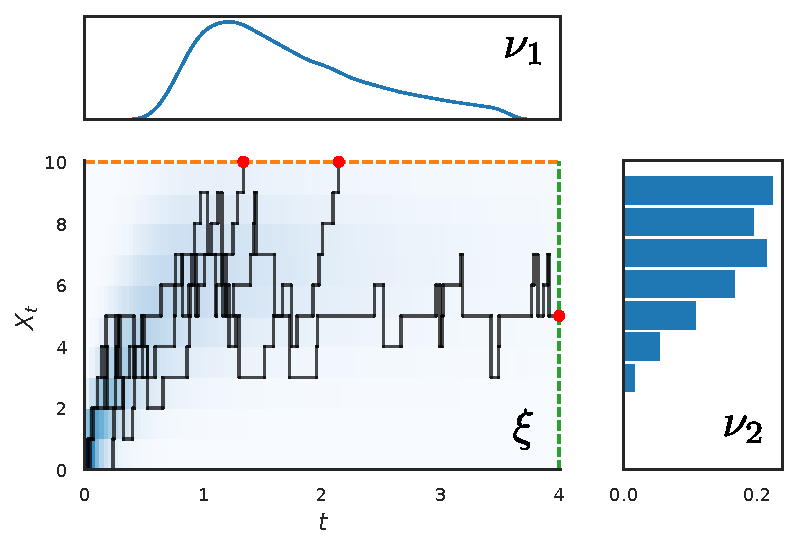
\includegraphics[scale=.8]{gfx/decomp1.pdf}
	\caption[Occupation measure $\xi$ and
	exit location probability measures $\nu_1$ and $\nu_2$]{The relationship between the occupation measure $\xi$ and the
    exit location probability measures $\nu_1$ and $\nu_2$. The shaded area indicates
    the structure of the occupation measure. Three example trajectories are
    additionally plotted with
	their exit location highlighted. The plots are based on \num{10000} sample trajectories.}
    \label{fig:decomposition}
\end{figure}
\end{example}


Equation~\eqref{eq:constraint}  describes a relationship between
two measures~\parencite[][Chapter~9.2]{lasserre2010moments}:
\begin{description}
\item[Expected Occupation Measure] $\xi$ describes the expected residence time inside a subset of the state-space and time. As such it is supported on $[0,H]\times [0,T]$:
\begin{equation}\label{eq:ex_occ_measure}
    \xi(A\times C) \coloneqq \E{\int_{[0,\tau]\cap {C}}{1}_{\in A}(X_t)\,dt},
\end{equation}
\item [Exit Location Probability] $\nu$ gives the state probability associated with the stopping time $\tau$. Therefore it is supported on $(\{H\}\times[0,T]) \cup
([0,H]\times\{T\})$:
% \todo{this can also be dropped, ie.\ we don't set a time-horizon. should be fine if passage time moments are finite (also
% in the relaxation)}
\begin{equation}\label{eq:exit_loc_measure}
    \nu(A\times C)\coloneqq \Pr((X_{\tau},\tau)\in A\times C),
\end{equation}
\end{description}
where $A\times C$ is a measurable set, i.e.\ $A$ and $C$ are elements of the Borel $\sigma$-algebras on $[0,H]$ and $[0,T]$, respectively.

Using \autoref{fig:decomposition}, one can gain an intuition for these two measures.
The expected occupation measure is shaded in blue.
As the name implies $\xi(A\times C)$ tells us how much time  the process spends
in $A$ up
to $\tau$ restricting to the time instants belonging to $C$.
In particular, $\xi([0,H]\times [0,T])=\E{\tau}$.
The exit location probability $\nu$, while being a two-dimensional distribution, can be viewed as a composition of a density describing the time at which the process reaches $H$ (if it does) and a probability mass function on the states of the process if the time-horizon is reached without exceeding $H$.
We partition the measure $\nu$ into $\nu_1$ and $\nu_2$ by conditioning on $\tau=T$.
Thus, 
\[
	\nu_1(C)\coloneqq\Pr(\tau\in C, \tau<T)
\]
and
\[
	\nu_2(A)\coloneqq\Pr(X_T\in A, \tau=T)
\]
and hence $\nu(A\times C)=\nu_1(C)+\nu_2(A)$.
To refer to the moments of these measures, we define \emph{partial moments}
\[
    \E{g({X}); f({Y}) = y}\coloneqq
    \E{g({X})\mid f({Y})=y}\Pr(f({Y})=y)\,,
    \]
for some polynomial $g$ and some indicator function $f$. Then
\[
	\E{\tau^k X_{\tau}^m}=T^k\E{X_{\tau}^m;\tau=T} + H^m\E{{\tau}^k;\tau < T, X_{\tau}=H}\,.
\]
% The partial expectations in terms of $\nu_1$, $\nu_2$
% \[
% \E{X_{\tau}^m;\tau=T} + \E{{\tau}^k;\tau < T, X_{\tau}=H}
% \]
Therefore the linear moment constraints are
\begin{multline}\label{eq:model_constraints}
 	0 = T^k\E{X_{\tau}^m;\tau=T} + H^m\E{{\tau}^k;\tau < T, X_{\tau}=H}\\
 	- 0^kx_0^{m}
 	% - k \E{\int_{0}^{\tau} t^{k-1} \vec X_t^m\,dt}
 	+ \sum_{i}c_i\E{\int_{0}^{\tau} t^{k_i}X_t^{m_i}\,dt}\,.
\end{multline}
% \begin{multline*}
% 	0 = \,&T^k\E{X_{\tau}^m;\tau=T} + H^m\E{{\tau}^k;\tau < T, X_{\tau}=H}\\
% 	- 0^kx_0^{m}
% 	% - k \E{\int_{0}^{\tau} t^{k-1} \vec X_t^m\,dt}
% 	+ \sum_{i}c_i\E{\int_{0}^{\tau} t^{k_i}X_t^{m_i}\,dt}\,.
% \end{multline*}
Next, we consider infinite sequences of partial moments 
 $\vec{y}_1=(y_{1k})_{k\in\mathbb{N}}$, $\vec{y}_2=(y_{2m})_{m\in\mathbb{N}}$, and $\vec{z}=(z_{mk})_{(m,k)^{\T}\in\mathbb{N}^2}$
 of $\nu_1$, $\nu_2$, and $\xi$, respectively.
 In particular,
\begin{align*}
	y_{1k} &\coloneqq \E{{\tau}^k;\tau < T}\,,\\
	y_{2m} &\coloneqq\E{X_{\tau}^m;\tau=T}\,,
\intertext{and}
	z_{km} &\coloneqq\E{\int_0^{\tau}t^k X_t^m\,dt}\,.
\end{align*}

\section{Objective}
Given the above measures and their corresponding moments, we can
now identify the moments we are particularly interested in.
We formulate an optimization problem with variables corresponding 
to the moments defined above.
The \ac{MFPT} is exactly the zeroth moment of $\xi$,
\[
	z_{00}=\E{\int_0^{\tau}1_{\leq H}(X_t)\,dt} = \E{\tau}\,.
\]
Therefore $z_{00}$ corresponds to the objective of the optimization problem
that gives bounds for the \ac{MFPT}.
Furthermore, we can easily change the objective to the  
zeroth moment of $\nu_1$,
\[
	y_{10} = \E{\tau^0;\tau<T}=\Pr(\tau < T)\,.
\]
This moment is the probability of reaching
threshold $H$ before reaching time-horizon $T$. Since the target set can be more complex, this formulation can be used to perform model checking on a
wide variety of properties.

Moreover, it is possible to formulate objectives not directly corresponding to
a raw moment such as the variance~\parencite{sakurai2019bounding,dowdy2018bounds}.

\section{Linear Hausdorff Constraints}
Before discussing the semi-definite constraints which we will use for the remainder of this study, we will briefly discuss the Hausdorff moment constraints.
These constraints offer linear constraints on moments of bounded measures.
The Hausdorff moment problem is the question whether an infinite sequence $(m_0, m_1, \dotsc)$ is a sequence of moments
\[
	m_k = \int_{0}^{1} x^k\,d\mu(x), \quad \forall k\in\mathbb{N}
\]
for some Borel-measure supported on the unit interval $[0,1]$.

\citet{hausdorff} came up with a necessary condition that
\marginpar{See also \citet{feller} for additional details.}
\begin{equation}\label{eq:hausdorff}
    \int_0^1 x^\ell(1-x)^k\,d\mu(x) \geq 0, \quad \forall \ell, k\in\mathbb{N}\,.
\end{equation}
The validity of this condition is easy to see since
\begin{equation}\label{eq:hausdorff_integrand}
	x^\ell(1-x)^k\geq 0, \quad \forall x\in[0,1]\,.
\end{equation}
Expanding this term yields a polynomial, which --~by integration~-- provides a linear constraint on the moments.
This moment condition has been used by \citet{helmes2001computing} to bound \acp{MFPT} in a variety of stochastic processes.
In \citet{helmes2008geometrical} the authors provide an extension taking into account the geometry of the Hausdorff polytope.
With this extension the method was competitive with the \ac{SDP} approach on their selection of case studies.
Since these conditions are linear in the moments they can solve \acp{LP} instead of the semi-definite programs shown below.

\begin{example}
	Let $\ell = 2$, $k=2$. Then the \eqref{eq:hausdorff} becomes
	\[
		\int_0^1 x (1 - x)^2 \,d\mu(x) =
		m_2 - 2 m_3 + m_4 \geq 0
	\]
	constraining the moments on $[0,1]$.
\end{example}

Since the Hausdorff moment problem is defined on $[0,1]$, we need to adjust accordingly.
Let the interval be $[0,H]$, $H>0$ then we can simply change the variables.
That means considering $y=x/H$ instead of $x$.
Equivalently, we can apply this rescaling in \eqref{eq:hausdorff} such that
\begin{equation}\label{eq:hausdorff_scaled}
	\int_0^H x^\ell(H-x)^k\,d\mu(x) \geq 0, \quad \forall \ell, k\in\mathbb{N}
\end{equation}
remains a valid constraint on $[0,H]$.

Generalizing \eqref{eq:hausdorff} to multiple dimensions can be done by simply multiplying terms
for each dimension in a similar manner.
For $n$ dimensions
\begin{equation*}
	\int_{{[0,1]}^n}\prod_{i = 0}^n x_i^{\ell_i}{(1-x_i)}^{k_i}\,d\mu{(\vec{x}})\geq 0
\end{equation*}
Using multi-index notation
\begin{equation*}
	\int_{{[0,1]}^n} x^{\vec{\ell}}{(\vec{1}-\vec{x})}^{\vec{k}}\,d\mu{(\vec{x}})\geq 0
\end{equation*}
for all $\vec\ell, \vec{k}\in\mathbb{N}^{n}$.
We treat the time horizon $T$ exactly the same as the other bounds $H_i$ here.
With arbitrary positive upper bounds $\vec{H} = (H_1, H_2, \dotsc, H_n)^{\T}$ this becomes
\begin{equation}\label{eq:hausdorff_constraint}
    \int_{\bigtimes_{i=1}^n[0,H_i]} x^{\vec{\ell}}{(\vec{H}-\vec{x})}^{\vec{k}}\,d\mu{(\vec{x}})\geq 0
\end{equation}
This equation can simply be expanded using the multi-binomial theorem. % Taken from Wikipedia : https://en.wikipedia.org/wiki/Binomial_theorem#Multi-binomial_theorem
This is just a vector version of the regular binomial theorem
That is, given $n$-dimensional vectors $k$, $x$, and $y$
\[
    (\vec{y}+\vec{x})^{\vec k} =
    \sum_{\vec j\leq\vec k}
    \binom{\vec k}{\vec j} {\vec{y}}^{\vec j}\vec{x}^{\vec k-\vec j}\,.
\]
% In multi-index notation
% \[
%     (y + x)^k = \sum_{\nu\leq k} \binom{k}{\nu} y^{\nu}x^{k-\nu}\,.
% \]
Thus, \eqref{eq:hausdorff_constraint} becomes the linear moment constraint
\begin{equation}\label{eq:hausdorff_appl}
    %\sum_{j_1=0}^{k_1}\dotsm\sum_{j_n=0}^{k_n}
    \sum_{\vec j\leq \vec k}
    %\left(\prod_{i=1}^{n}\binom{k_i}{j_i}
    \binom{\vec{k}}{\vec j}
    %H_i^{j_i}(-1)^{k_i-j_i}
    {\vec{H}}^{\vec{j}} (-1)^{\vec k-\vec j}
    %\right)\\
    %\int_{\bigtimes_{i=1}^n[0,H_i]}
    \int
    {\vec x}^{\vec k-\vec j+\vec \ell} \,d\mu(\vec x)\geq 0\,.
\end{equation}
We can interchange the integrals since all measures have finite support and mass.

\subsection{A Linear Program}
Combining the model constraints \eqref{eq:model_constraints} and the linear Hausdorff-type constraints \eqref{eq:hausdorff_appl} for both expected occupation and the exit location measure yields a \ac{LP}.
\begin{equation}\label{eq:lp_for_fpt}
    \begin{split}
	    \text{min} / \text{max} \hspace{1em}&  z_{00}^{\prime} \\
        \text{such that}\hspace{1em} & \text{for all measures and bounds}\\
        &\qquad\eqref{eq:hausdorff_appl}\text{ holds }\forall m, k,\\
        & 0= y_{1k}' H^m -  y_{2m}'T^k - 0^k x_0^m \\
	    &\qquad\quad+\sum_i c_i  z_{k_i m_i}', \quad\forall m, k\,.
    \end{split}
\end{equation}
Using a framework such as \acsfont{CVXPY}, this convex program can easily be coded and solved using various state-of-the-art solvers.

\section{Semi-Definite Constraints}
The linear constraints alone are not sufficient to identify moment bounds.
We further leverage the fact that a necessary condition for a positive measure that the \emph{moment matrices}
are positive semi-definite.
A matrix $M\in\mathbb{R}^{n\times n}$ is positive semi-definite, denoted by  $M\succeq 0$ if and only if
\[
	{\vec v}^T M{\vec v} \geq 0\quad \forall \vec v\in\mathbb{R}^n\,.
\]
\begin{example}
As an example, let us consider a one-dimensional random variable $Z$
with moment sequence $\vec z$.
For  moment order $r$,
the entries of the $(r+1)\times (r+1)$ moment matrix $M_r(\vec x)$ are given by
the raw moments.
In particular, 
\[ 
	(M_r({\vec{z}}))_{ij}=z_{i+j-2}=\E{Z^{i+j-2}}
\]
for
$i,j\in\mathbb{N}_r$ where $\mathbb{N}_r=\{0,1,\dots,r\}$ and the maximum order in the matrix is $2r$.
For instance,
\begin{equation}
\label{eq:m1_dim}
    M_1(\vec x) =
    \begin{bmatrix}
    x_0 & x_1 \\
    x_1 & x_2
    \end{bmatrix}
\end{equation}
needs to be positive semi-definite. By Sylvester's criterion this means $\det
M_1\geq 0$ and $x_0\geq 0$.
We can easily see that in this case this entails
	\[
\det M_1=x_0x_2 - x_1^2=\E{X^2}-\E{X}^2
=\Var({X})
\geq 0\,.
\]
This restriction is natural since the variance cannot be negative.
\end{example}
% Even though the measures $\nu_1$, $\nu_2$, and $\xi$ are not probability measures
% this restriction remains valid for them. Either they can be normalized to
% form a probability measure, or if their mass is zero % we don't care...
The restriction of the non-negative variance we saw in the example generalizes
to moment matrices in form of a positive semi-definite constraint \parencite{parrilo2003semidefinite}.\graffito{This constraint is valid for general positive measures --- even if they do not model probabilities.}
This gives us the following restrictions on the moment matrices.
\begin{equation}\label{eq:sd_constraints}
M_r(\vec{z})\succeq 0, \quad M_r(\vec{y_1})\succeq 0,\quad\text{and}\quad M_r(\vec{y_2})\succeq 0
\end{equation}
for arbitrary orders $r$, providing a first tranche of moment constraints.

Furthermore, we need to enforce the restriction of the measures $\xi$, $\nu_1$, and $\nu_2$
to their supports.
This can be done, by defining non-negative polynomials
on the intended support of the measure.
\begin{example}
The exit location probability $\nu_2$ has support $[0,H]$. We can now define
	\[
u_H(t,x) = Hx - x^2, \quad x\in \mathbb R
\]
as a polynomial that is non-negative on $[0,H]$.
Using such polynomials, we can construct \emph{localizing matrices},
which have to be positive semi-definite~\parencite{lasserre2010moments}.
Applying $u_H$ to the moment matrix of measure $\nu_2$, i.e.\ $M_1(\vec{y}_2)$
	\[
M_1(u_H, \vec{y_2})=
\begin{bmatrix}
    Hy_{21} - y_{22} & Hy_{22} - y_{23} \\
    Hy_{22} - y_{23} & Hy_{23} - y_{24}
\end{bmatrix}
\]
with the constraint $M_1(u_H, \vec{y_2})\succeq 0$, where the application of
a polynomial such as $u_H$ to a moment matrix
is formally defined for the multidimensional case in \autoref{subsec:mfpt:multidim}.
Similarly, let $u_T(t, x) = Tt-t^2$ to restrict $\nu_1$ to $[0,T)$.
The expected occupation measure $\xi$ is constrained similarly to its domain
$[0,H]\times[0,T]$.
This gives us the following restrictions on the moment matrices.
\begin{equation}\label{eq:localizing_sd_constraints}
\begin{split}
	& M_r(u_T,\vec{z})\succeq 0\,, &M_r(u_T,\vec{y_1})\succeq 0\,,\\
	& M_r(u_H,\vec{z})\succeq 0\,, &M_r(u_H,\vec{y_2})\succeq 0\,.
\end{split}
\end{equation}
\end{example}

\subsection{Multi-Dimensional Generalization}
\label{subsec:mfpt:multidim}
For a general multi-dimensional moment sequence
\[
	\vec{y}={\left(\E{\vec X^{\vec{m}}}\right)}_{\vec{m}\in\mathbb{N}^{n_s}}\,,
\]
	the moment
matrix is~\parencite{lasserre2010moments}
% \todo{explain the order $r$ in some detail (max order is $2r$), define
% $\mathbb{N}_r^n$}
\begin{equation}\label{eq:def_mom_mat}
	M_r(\vec y)(\vec\alpha,\vec\beta)
=y_{\vec\alpha + \vec\beta},\quad\forall\vec{\alpha},
\vec{\beta}\in\mathbb{N}_r^n
\end{equation}
where row and column indices, $\vec{\alpha}$ and $\vec\beta$, are ordered according to the canonical basis
\begin{multline}\label{eq:canoncial_basis}
\vec{v}_r(\vec{x}) =
(1,x_1,x_2,\dots,x_n,x_1^2,x_1x_2,\dots \\
	\dots, x_1x_n,\dots ,x_1^r,\dots
	,x_n^r)^T\,.
\end{multline}
Equivalently to \eqref{eq:def_mom_mat},
\[
	M_r(\vec{y})=\E{\vec{v}_r (\vec x)\vec{v}_r(\vec x)^T}\,.
\]
For a moment sequence the semi-definite restriction $M_r(\vec{y})\succeq 0$ must hold.

Measures can be restricted to semi-algebraic sets
\[
	\{\vec x\in\mathbb{R}^n \mid u_j(\vec x)\geq 0, j=1,\dots,m\}\,,
\]
where $u_j$, $j=1,\dots,m$ are polynomials~\parencite{lasserre2010moments}.
This is done by placing restrictions on the {localizing matrices}.
For each polynomial $u_i\in\mathbb{R}[x]$ with coefficient vector
$\vec{u}=\{u_{\vec\gamma}\}$,
i.e.\ \[u(\vec x) = \sum_{\vec{\gamma}\in\mathbb{N}^n} u_{\vec{\gamma}}
\vec{x}^{\vec{\gamma}}\,,\]
the localizing matrix is
\[ M_r(u, \vec{y})(\vec{\alpha}, \vec{\beta})=
\sum_{\vec\gamma\in\mathbb{N}^n}u_{\vec\gamma}
y_{\vec\gamma+\vec\alpha+\vec\beta},\quad
\forall\vec{\alpha},\vec{\beta}\in\mathbb{N}^n_r.
\]
Requiring that this matrix is positive semi-definite restricts the measure to
$\{\vec{x}\mid u_i(\vec{x})\geq 0\}$.
This way we can, for example, restrict the moment sequence $\vec{y}$
to measures that are positive w.r.t.\ dimension $j$.
Simply letting $u(\vec{x}) = x_j$ and requiring
$M_1(\vec{u},\vec{y})\succeq 0$ for $i=1,\dots,n_S$ gives us this restriction.


\subsection{A Semi-Definite Program}
With the linear constraints given in \eqref{eq:constraint}
and the semi-definite constraints \eqref{eq:sd_constraints} and \eqref{eq:localizing_sd_constraints} 
discussed in the previous sections, we can now formulate a
\acf{SDP} for any relaxation order $0<r<\infty$.
An \ac{SDP} is a convex optimization problem over the set of positive semi-definite $n \times n$-matrices
$\mathcal{X}$ under linear constraints:
\begin{equation}
    \label{eq:sdp_canonical}
    \begin{split}
        \min_{X\in\mathcal{X}} \hspace{1em} & \sum_{i,j} A_{ij}^{(0)}X_{ij} \\
        \text{such that} \hspace{1em}
                 & X\succeq 0\\
            & \sum_{i,j} A_{ij}^{(k)}X_{ij} \leq b_k, \quad k=1,\dots,m
    \end{split}
\end{equation}
with constant matrices $A^{(i)}\in \mathbb{R}^{n\times n}$, $i=0,\dots,m$ and
constants $b_k\in\mathbb{R}$, $k=1,\dots,m$ to define a set of $m$ linear constraints.
Such a problem is convex and can be solved efficiently using off-the-shelf solvers~\parencite{vandenberghe2010cvxopt}.

With each moment sequence $\vec x$ we associate a sequence proxy variables $\vec{x'}$
used in the optimization problem.
\begin{equation}\label{eq:sdp_for_fpt}
    \begin{split}
	    \text{min} / \text{max} \hspace{1em}&  z_{00}^{\prime} \\
        \text{such that}\hspace{1em} & M_r(\vec{z'})\succeq 0,
                   M_r({u}_T, \vec{z'})\succeq 0, M_r({u}_H, \vec{z'})\succeq 0,\\
        & M_r(\vec{y_1'}) \succeq 0, M_r({u}_T,\vec{y_1'}) \succeq 0,\\
        & M_r(\vec{y_2'}) \succeq 0, M_r({u}_H, \vec{y_2'}) \succeq 0,\\
        & 0= y_{1k}' H^m -  y_{2m}'T^k - 0^k x_0^m \\
	    &\qquad\quad+\sum_i c_i  z_{k_i m_i}', \quad\forall m, k\,.
    \end{split}
\end{equation}
This \ac{SDP} can be compiled to the canonical form.
To this end, the moment matrices can be arranged in a block-diagonal form and the
localizing constraints \eqref{eq:localizing_sd_constraints} can be encoded
by the introduction of new variables and appropriate equality constraints.
This transformation can be done automatically using modeling frameworks
such as \acsfont{CVXPY}~\parencite{cvxpy}. We therefore only give the \ac{SDP} in the more intuitive format.
This problem can be solved using off-the-shelf \ac{SDP} solvers such as \acsfont{MOSEK}~\parencite{mosek},
\acsfont{CVXOPT}~\parencite{vandenberghe2010cvxopt}, or \acsfont{SCS}~\parencite{scs}.

In principle, we can choose an arbitrarily large order $r$ for the moment matrices
and their corresponding constraints, because there are
infinitely many moments.
In practice, however, the order is bounded by practical issues such as the program size
(number of constraints and variables) and numerical issues.
These issues are discussed in \autoref{sec:mfpt:evaluation} in more detail.
Choosing a finite $r$ is a relaxation of the problem since it removes constraints regarding
higher-order moments.


\section{Implementation \textit{\&} Evaluation}\label{sec:mfpt:evaluation}
The implementation of the \ac{SDP} \eqref{eq:sdp_for_fpt} is straightforward using
modeling frameworks and off-the-shelf solvers.
However, as noted in previous work~\parencite{dowdy2018dynamic,sakurai2017convex,dowdy2018bounds,sakurai2019bounding} on moment-based \acp{SDP}
the direct implementation of the problem may lead to difficulties for the solver.
A source of these is that moments of various orders by nature
may differ by many orders of magnitude.
A re-scaling of the moments~\parencite{dowdy2018bounds,sakurai2019bounding}
such that moments only vary by few orders of magnitude
may alleviate this problem.
In other scenarios such as the bounding of general transient or steady-state moments,
the scaling can be particularly difficult,
because the magnitude of moments is generally not known
a priori. In the context of \acp{MFPT} with a finite time-horizon
moments are trivially bounded.

\subsection{Moment Scaling}\label{sec:mfpt:scaling}
Using the fact that
$\mathcal{S}\setminus {B}$ is often finite,
it is possible to derive trivial bounds, which can be used to scale moments.
If, for example, we have a one-dimensional process $X_t$ with $X_0 = 0$ a.s.\ and are interested in the hitting
time of an upper threshold $H>0$ until time $T>0$ for $i,k\in \mathbb N$
\begin{multline*}
z_{ik} = \E{\int_0^{\tau}t^i X_t^k\,dt}\leq\E{\int_0^T t^i X_t^k\,dt}\\\leq H^k\int_0^T t^i\,dt
=\frac{T^{i+1}H^k}{i+1}\,.
\end{multline*}
Thus, we fix a scaling vector $\vec d$ with entries $d_{ik}={T^{i+1}H^k}$ in
the same order
as the canonical base vector~\eqref{eq:canoncial_basis}.
Using this scaling vector, we can define a scaling
matrix $D={\vec d}{\vec{d}}^{\T}$.
Clearly, $D \succeq 0$.
Now we can formulate the optimization~\eqref{eq:sdp_for_fpt}
over a scaled version $D^{-1}M(\vec{z'})$ instead of $M(\vec{z'})$.
The moment matrices of the exit location probabilities are scaled in the same
way.
\graffito{These scaling strategies have not been evluated so far.}
Alternatively, one could use approximations such as moment closures
or bounds obtained by lower-order relaxations or solve a sequence
of problems, incrementally increasing
the time-horizon, and adjust the scaling accordingly (suggested in \citet{dowdy2018dynamic}).

In \autoref{fig:magnitudes} we illustrate the influence the scaling has on the
optimization variables. While the unscaled version shows large differences
between values, these differences become significantly smaller in the scaled version
of the problem.
\begin{figure}[htb]
    \centering
    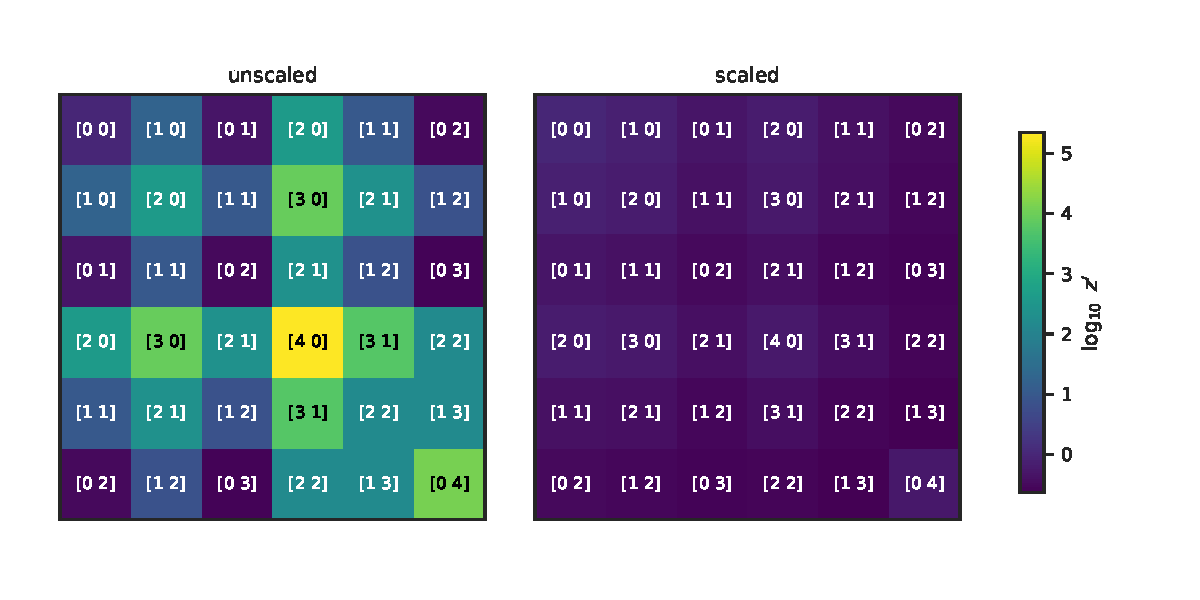
\includegraphics[width=\textwidth]{gfx/magnitudes.pdf}
	\caption[Moment matrix scaling]{The unscaled and scaled value of the moment matrix proxy variable
    $M(\vec{z'})$ after optimization using \acsfont{MOSEK}. The indices are given along the
    logarithmic (base $10$) values. The unscaled version (left) shows large
    differences in magnitudes, while on the scaling suppresses
    these large variations (right). The case study used here is \autoref{model:dim},
    with a threshold $H=25$ for species $M$ and a time-horizon $T=1$. The
    relaxation order $r=2$. Therefore moments of orders up to $2r=4$ appear.}
    \label{fig:magnitudes}
\end{figure}


\subsection{Case Studies}
The model constraints are derived using the symbolic math toolkit Sympy \parencite{sympy}.
The \acp{LP} are solved using the Gurobi \parencite{gurobi}.
We implemented and solved the \ac{SDP} programs described above using optimization suite \acsfont{MOSEK} version 9.1.2 \parencite{mosek}.
Both optimizers are used through the \acsfont{CVXPY} interface \parencite{cvxpy}.

\subsubsection*{Dimerization}
As a first case study, we use \autoref{model:dim} with parameters $\lambda=100$ and $\delta=0.2$.
In this model, we are interested in the time at which the number of agents of type $M$
surpasses a threshold of $25$ before some time-horizon $T$,
i.e.\ \[
	\tau=\inf\{t\geq 0\mid X_t \geq 25\}\land T\,.
\]
First, we set no finite time-horizon $T$, i.e.\ $T=\infty$.
\marginpar{We can let $T\to\infty$ because this system is ergodic and therefore $\tau<\infty$ a.s.}
This is achieved by dropping the moments $\vec y_2$
of measure $\nu_2$ in the linear constraints~\eqref{eq:sdp_for_fpt}.
This can be done because the threshold on $M$ makes the state-space finite
and therefore the first passage time distribution is a phase-type distribution
which possesses finite moments \parencite[][Chapter 7.6]{stewart2009probability}.

The empirical \ac{FPT} distribution based on \num{100000} \ac{SSA} simulations is given in \autoref{fig:dim_fpt_fpt}
and the bounds, given different moment orders, are given in \autoref{fig:dim_fpt:mfpt}.
As we can see in \autoref{fig:dim_fpt:mfpt}, the bounds capture the \ac{MFPT} precisely for orders \numlist{5;6}.
The difference between upper and lower bound decreases roughly exponentially with increasing relaxation order $r$.
We found that this trend was consistent among the case studies presented here (cf.\ \autoref{fig:convergence}).
\begin{figure}
	\centering
	\subfloat[\ac{FPT} distribution]
    {\label{fig:dim_fpt_fpt}
	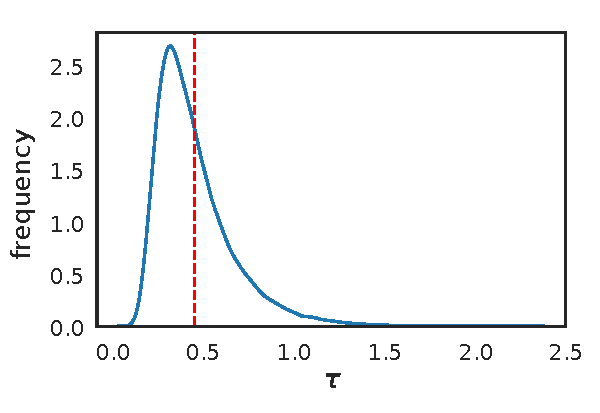
\includegraphics[width=.48\textwidth]{gfx/fpt_dist_dim.pdf}}
	\subfloat[\ac{MFPT} bounds.]
    {\label{fig:dim_fpt:mfpt}%
        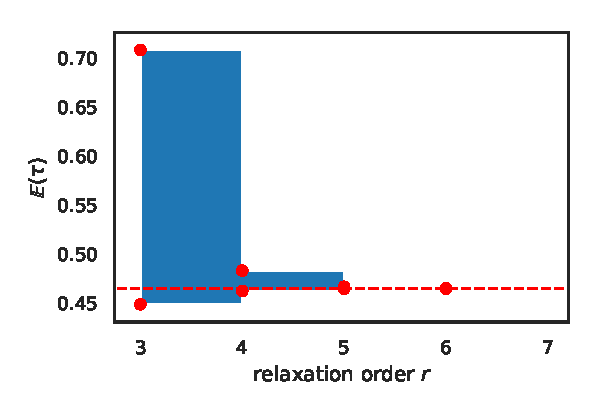
\includegraphics[width=.48\textwidth]{gfx/fpt_bounds_dim.pdf}} \\
	\caption[\ac{FPT} and \ac{MFPT} distribution and bounds]{First-passage time characterisitics for \autoref{model:dim} with $\tau=\inf\{t\geq 0\mid X_t \geq 10\}\land \infty$.
	The dashed red line denotes the sampled \ac{MFPT} based on \num{100000} \ac{SSA} samples. Bounds are based on the \ac{SDP} \eqref{eq:sdp_for_fpt} with different moment orders}
\end{figure}
% \begin{figure}[t]
%     \centering
%     \begin{minipage}{.49\textwidth}
%     \centering
%     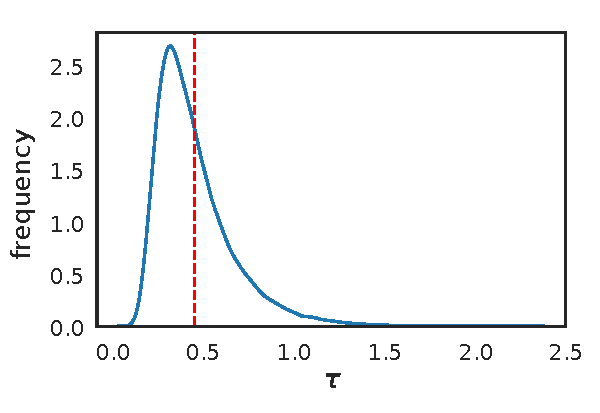
\includegraphics[scale=.6]{gfx/fpt_dist_dim.pdf}\\(a)
%     \end{minipage}
%     \begin{minipage}{.49\textwidth}
%     \centering
%     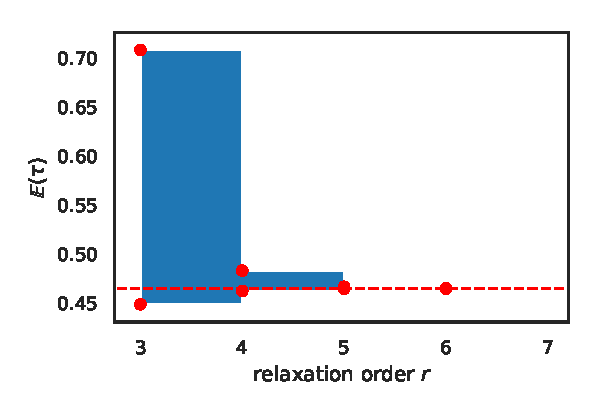
\includegraphics[scale=.6]{gfx/fpt_bounds_dim.pdf}\\(b)
%     \end{minipage}
% 	\caption{    (a) The distribution of $\tau$ estimated based on 100,000 \ac{SSA} samples.
%     (b) The bounds based on the \ac{SDP} in~\eqref{eq:sdp_for_fpt} with different moment
%     orders.\label{fig:dim_fpt}}
% \end{figure}

Next, we look at first passage times within a finite time-horizon $T$.
In \autoref{fig:dim_fpt_fin:mfpt} we summarize the bounds obtained for the \ac{MFPT} over $T$.
While low-order relaxations (light) give rather loose bounds, the bounds are already fairly tight
when using $r=4$.
In many cases, hitting probabilities, that is, the probability of reaching the
threshold before time $T$, are of particular interest.
This is done by switching the optimization objective in~\eqref{eq:sdp_for_fpt} from the mass of the
expected occupation measure $\xi$ to the mass of $\nu_1$.
In terms of moments, the objective changes from $z_{00}$ to $y_{10}$.
The need for such a scenario often aris\-es in the context of model checking, where one might be
interested in the probability of a population exceeding a critical threshold.
By varying the time-horizon, we are able to recover bounds on the cumulative density 
\[
	F(t) = \Pr(X_s=H\mid s<t)
\]
of the first passage time (\autoref{fig:dim_fpt_fin:rp}).
\begin{figure}
    \centering
	\subfloat[\ac{MFPT} bounds over $T$.]
    {\label{fig:dim_fpt_fin:mfpt}
	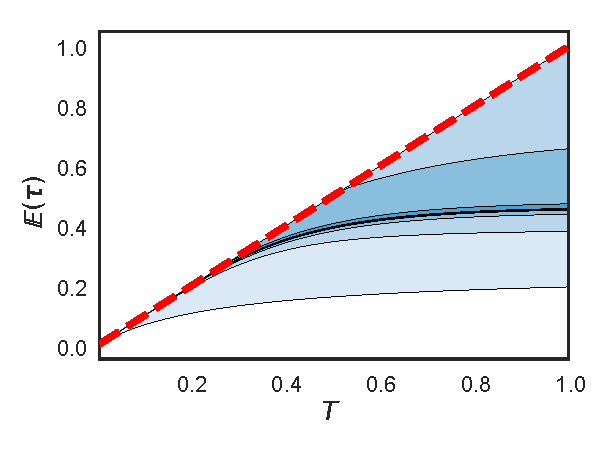
\includegraphics[width=.48\textwidth]{gfx/mfpt_bounds.pdf}}
    \subfloat[Reaching probabilities up to $T$.]
    {\label{fig:dim_fpt_fin:rp}
        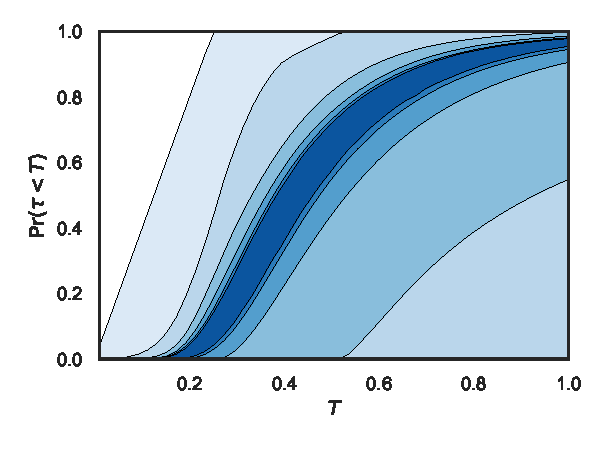
\includegraphics[width=.48\textwidth]{gfx/reachability_probs.pdf}}
	\caption[\acp{MFPT} up to a varying time-horizon]{\Acp{MFPT} and reaching probability bounds for the dimerization model with
    $\tau=\inf\{t\geq 0\mid X_t \geq 25\}\land T$ and varying $T$.
	The results for \ac{SDP} relaxations of orders \num{1} (light) to \num{6} (dark) are shown.\label{fig:dim_fpt_fin}}
\end{figure}
% \begin{figure}[t]
%     \centering
%     \begin{minipage}{.49\textwidth}
%     \centering
%     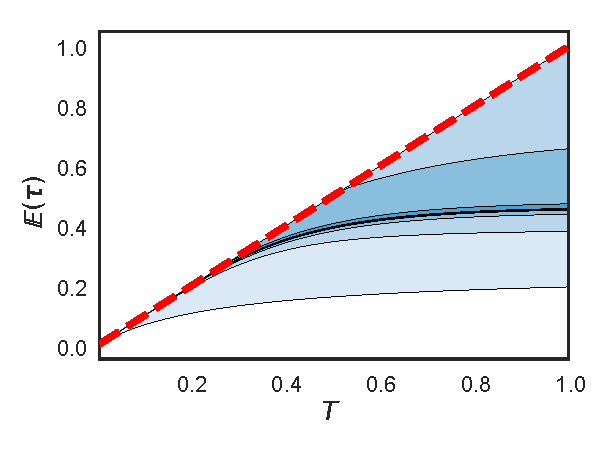
\includegraphics[scale=.6]{gfx/mfpt_bounds.pdf}\\(a)
%     \end{minipage}
%     \begin{minipage}{.49\textwidth}
%     \centering
%     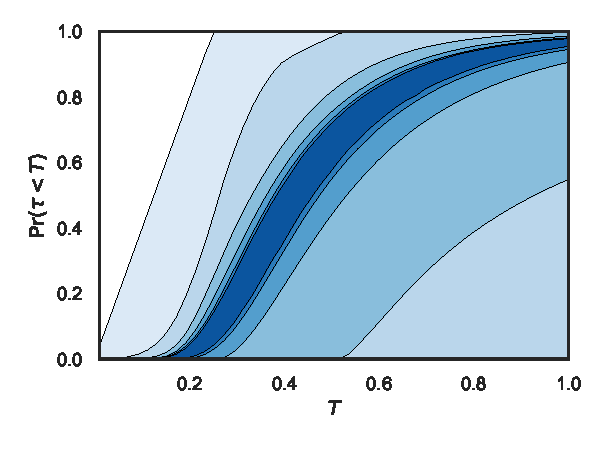
\includegraphics[scale=.6]{gfx/reachability_probs.pdf}\\(b)
%     \end{minipage}
%     % \begin{minipage}{.15\textwidth}
%     % legend
%     % \end{minipage}
%     \caption{First passage times for the dimerization model with
%     $\tau=\inf\{t\geq 0\mid X_t \geq 25\}\land T$.
%     The results for \ac{SDP} relaxations of orders \num{1} (light) to \num{6} (dark) are shown.
%     (a) The bounds on the \ac{MFPT} for differing time-horizons $T$.
%     (b) Bounds on the probability to reach the threshold before time $T$.\label{fig:dim_fpt_fin}}
% \end{figure}

Finally, we look at turn to the dimer species $D$ that is synthesized by the combination of
two monomers $M$. Here, we look at the time until the agents of type $D$ exceed a threshold of five
with a time-horizon $T=1$. Note that we do not limit the number of $M$ agents. Therefore
the analyzed state-space is countably infinite. As in the previous two examples, we
observe a roughly exponential decrease in interval size with increasing relaxation
order $r$ (cf.\ \autoref{fig:convergence} and \autoref{tab:bounds}).


\subsubsection*{Parallel Dimerizations}
As a second study, we consider a two-dimensional model by combining two
independent dimerizations.
\begin{model}[Parallel Independent Dimerizations]\label{model:double_dim} This model consists of two independent versions of \autoref{model:dim}\turnto{model:dim}. The reactions are
\[
    \varnothing\xrightarrow{10^4}M_1\,,\quad
    2M_1\xrightarrow{0.1}D_1\,,\quad
    \varnothing\xrightarrow{10^4}M_2\,,\quad
    2M_2\xrightarrow{0.1}D_2\,.
\]
Initially, \[0=X_0^{(M_1)}=X_0^{(M_2)}=X_0^{(D_1)}=X_0^{(D_2)}\,.\]
\end{model}
As a \ac{FPT} we consider the time at which either $M_1$ or $M_2$ surpasses a threshold of \num{200} or a time-horizon of $T=10$
is reached, i.e.
\[ \tau=\inf\{t\geq 0\mid X_t^{(M_1)} \geq 200\}\land \inf\{t\geq 0\mid X_t^{(M_2)} \geq 200\}\land 10\,.
\]
As before, we ignore the product species $D_1$ and $D_2$ since they do not influence $\tau$.
% Still, the possible state-space reaches a size of $200^2=\num{40000}$.
% \luca{40000 is very small... I would not emphasize it}\todo{yes, but the only reason for this case study ist that we have a ``larger'' relevant state-space}
The \ac{SSA}   (using $n=\num{10000}$ runs) gives the estimate $\E{\tau}\approx {0.028378}$ %\pm 1.3025e-04$ (99\%-CI)
which is captured tightly by the \ac{SDP} bounds (cf.\ \autoref{tab:bounds}).
For higher relaxation orders $r \geq 5$  numerical issues prevented the solution of the
corresponding \acp{SDP}.

\subsection{Hybrid Models \textit{\&} Multi-Modality}
The analysis of switching times is a particularly interesting case of \acp{FPT} that
arises in many   contexts.
Often mode switching in such systems can be described a modulating Markov process
whose switching rates may depend on the system state (e.g.\ the population sizes).
In biological applications, mode switching often describes a change of the
\acsfont{DNA} state~\parencite{hasenauer2014method,stekel2008strong} and the analysis of
switching time distribution is of particular interest~\parencite{spieler2014model,barzel2008calculation}.

In the context of \acp{MPM}, typically the state-space $\mathcal{S}=
\mathbb{N}^{\tilde{n}_S}\times {\{0,1\}}^{\hat{n}_S}$.
This state is modeled by  $\hat{n}_S$ population variables with
binary domains. Therefore, at each time point, the state of these modulator variables
is given by a set of Bernoulli random variables.
When considering the moments of
such a variable $X$, clearly
\[
	\E{X^m}=\E{X}=\Pr(X=1)\,,\quad \forall m\geq 1
\]
We can use this fact two ways: We could use the same moment
constraints
as above and impose additional equality constraints on the moments matrices
to ensure $\E{X^m}=\E{X}$, $m\geq 1$.
Alternatively, we can apply this simplification to the moment equation, which we choose here.

We apply a  split of variables $\vec X_t$  into the high count part ${\vec{\tilde{X}}}_t$ and the binary
part ${\vec{\hat{X}}}_t$ to
the expectations in~\eqref{eq:mfpt:mom_ode}. Similarly, we split   $\vec v_j$ and
with a case
distinction over the mode variable,
we arrive at a similar result as in~\parencite{hasenauer2014method}:
\begin{equation}\label{eq:mcm}
\begin{split}
	& \frac{d}{dt}\E{\vec{\tilde{X}}^{{\vec m}}_t 1_{=\vec y}({\vec{\hat{X}}}_t)}\\
   =&\sum_{j=1}^{n_R}
   \E{\left(\left(\vec{\tilde{X}}_t+\vec{\tilde{v}}_j\right)^{\vec
   m}1_{=\vec y}({\vec{\hat{X}}}_t+\vec{\hat{v}}_j)
       -{\vec{\tilde{X}}}_t^{\vec
       m}1_{=\vec y}({\vec{\hat{X}}}_t)\right)\alpha(\vec X_t) }\\
    =&\sum_{j=1}^{n_R}
        \E{{\left(
                {\vec{\tilde{{X}}}}_t+\vec{\tilde{{v}}}_j
            \right)}^{\vec{m}}\alpha_j(\vec{\tilde{{X}}}_t, \vec{{y}} -
            \vec{\hat{v}}_j)
            1_{={\vec{y}- \vec{\hat{v}}_j}}({\vec{\hat{X}}}_t )}\\
    &\quad- \sum_{j=1}^{n_R}
    \E{{\vec{\tilde{{X}}}}_t^{\vec{m}}\alpha_j(\vec{\tilde{{X}}}_t,
                {\vec{y}})
            1_{=\vec y}({\vec{\hat{X}}}_t)}\,.
            \end{split}
\end{equation}
Similarly to the general moment case, we can derive a constraint, by multiplying with a time-weighting factor
and integrating.

For simplicity, here we assume $\tilde n_S=\hat n_S=1$.
Fixing appropriate sequences ${(c_i)}_i$, ${(m_i)}_i$, ${(k_i)}_i$, and
${(y_i)}_i$ the constraint has the following form.\graffito{We fix $0^0=1$.}
\begin{equation}\label{eq:mcm_constraint}
    \begin{split}
	    &\sum_{y\in\{0,1\}}{H}^{m}\E{\tau^k;{{\hat{X}}}_{\tau}= y, \tau
    < T}\\ &\qquad\quad+ T^k\E{{{\tilde{X}}}_T^{m};{{\hat{X}}}_T= y,\tau=T}\\
      =\; &  0^k{{\tilde{x}}}_0^{m} 1_{=  y}({\hat{x}}_0) +
    \sum_i c_i %\sum_{y\in\{0,1\}}
        \E{\int_0^{\tau}t^{k_i}{{{\tilde{X}}}_t}^{{m}_i}\,dt;
            {{\hat{X}}}_t= y_i}\\
    \end{split}
\end{equation}
This way we can decompose the moment matrices such that for each mode $y\in\{0,1\}$,
we have moment matrices composed of the respective partial moments.
To this end, let $z^{(y)}_m$ be the partial moment w.r.t.\ ${{\hat{X}}}= y$.
The moment constraint over the partial moments has a linear structure:
\begin{equation}
0=y_{1k} {H}^{m} - y_{2m}T^k - 0^k x_0^{m}
+\sum_i c_i z^{(y_i)}_{k_i  m_i}\,.
\end{equation}

\begin{table}[t]
\centering
    \caption[\ac{MFPT} bounds]{\ac{MFPT} bounds on \autoref{model:dim} for $X_t \geq 5$ and $T=1$, \autoref{model:double_dim} for $X_t^{(M_1)}\geq 200$ or $X_t^{(M_2)}\geq 200$ and $T=10$, and \autoref{model:gexpr} for $X_t^{(P)}\geq 5$ and $T=10$.\label{tab:bounds}}
\begin{tabular}{l@{\hspace{1em}}l@{\hspace{1em}}r@{\hspace{2ex}}r@{\hspace{2ex}}r@{\hspace{2ex}}r@{\hspace{2ex}}r}
    \toprule
    & & \multicolumn{5}{c}{relaxation order $r$}\\
        \cmidrule{3-7}
        & & $1$ & $2$        & $3$        & $4$       & $5$       \\
        \midrule
        \autoref{model:dim} & lower & $0.0909$ & $0.2661$ & $0.2845$ & $0.2867$ & $0.2871$ \\
        & upper & $1.0000$ & $0.3068$ & $0.2932$ & $0.2886$ & $0.2875$  \\
         \midrule
         \autoref{model:double_dim} & lower & $0.0010$ & $0.0250$ & $0.0275$ & $0.0280$ & $0.0280$ \\
         & upper & $10.0000$ & $0.0575$ & $0.0323$ & $0.0299$ & $0.0290$ \\
         \midrule
         \autoref{model:gexpr} & lower & $4.0000$ & $6.0028$ & $6.2207$ & $6.3377$ & $6.3772$  \\
         & upper & $10.7179$ & $6.4619$ & $6.4079$ & $6.4004$ & $6.3835$ \\\bottomrule
\end{tabular}
\end{table}

\subsubsection*{Gene Expression with Negative Feedback}
As an instance of a multi-modal system, we consider a simple gene expression with self-regulating
negative feedback which is a common pattern in many genetic circuits~\parencite{stekel2008strong}.

\begin{model}[Negative Self-Regulated Gene Expression]\label{model:gexpr}
This model consists of a gene state that is either on or off, i.e.\ $X^{D_{\text{on}}}_t
+X^{D_{\text{off}}}_t = 1$, $\forall t\geq 0$. Therefore the system has two \emph{modes}.
\begin{gather*}
    D_{\text{on}} \xrightarrow{\tau_{0}} D_{\text{off}}\,, \quad
    D_{\text{off}} \xrightarrow{\tau_{1}} D_{\text{on}}\,, \quad
    D_{\text{on}} \xrightarrow{\rho} D_{\text{on}} + P \,, \\
    P\xrightarrow{\delta}\varnothing\,,\quad
    P + D_{\text{on}} \xrightarrow{\gamma} D_{\text{off}}\,.
\end{gather*}
The model parameters are $(\tau_0,\tau_1,\rho,\delta,\gamma)=(10,10,2,0.1,0.1)$ and
$X_0^{(D_{\text{off}})}=1$, $X_0^{(P)}=0$ a.s.
\end{model}

As a first passage time we consider 
\[
	\tau=\inf\{t\geq 0\mid X_t^{(P)} \geq 5\}\land 20\,.
\]


The results are summarized in \autoref{tab:bounds}.
The estimated \ac{MFPT} based on \num{100000}
\ac{SSA} samples is $\E{\tau}\approx 6.37795\pm0.02847$ at $99\%$ confidence level.
Note that our \ac{SDP} solution for $r=5$ yields tighter moment bounds than
the statistical estimation.% based on $100,000$ trajectories.


In \autoref{fig:convergence} we summarize our results about the decrease of the interval widths for increasing relaxation order $r$ by plotting them on a log-scale.
We see an approximately exponential decrease with increasing $r$.
The \acp{SDP} above were all solved within at most a few seconds.
\begin{figure}[t]
    \centering
    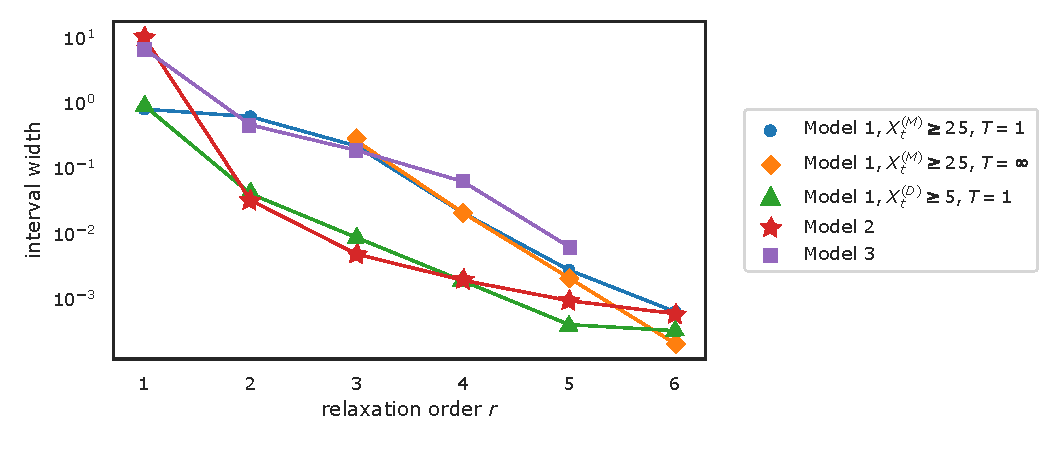
\includegraphics[width=\textwidth]{gfx/convergence.pdf}
	\caption[\ac{MFPT} bound convergence]{The interval width, i.e.\ the difference between upper and lower bound,
    for different case studies and targeted first passage times against the order $r$
    of the \ac{SDP} relaxation.\label{fig:convergence}}
\end{figure}



\section{Conclusion}\label{sec:mfpt:conclusion}
Numerical methods to compute reachability probabilities and first passage times
for continuous-time Markov chains that are based on an exhaustive exploration of the state-space
are exact up to numerical precision. Such methods, however, do not scale and cannot be efficiently applied to models with large or infinite state-spaces,
an issue exacerbated in population models. Moment-based methods offer an alternative analysis approach
for \acp{MPM}, which scales with the number of different populations in the system
but are approximations with little or no control of the error.
In this work,
we bridge this gap by proposing a rigorous approach to derive bounds on first passage
times and reachability probabilities, leveraging a semi-definite programming formulation
based on appropriate moment constraints. 

The method we propose is shown to be accurate in several examples. It does, however, suffer, like all moment-based methods, from numerical instabilities in the \ac{SDP} solver, caused by the fact that moments typically span several orders of magnitude. We proposed a scaling of moments to mitigate this effect. 
However, the scaling only addresses the moment matrices but not the linear constraints
which still contain values with varying orders of magnitudes.
Therefore, we plan as future work to investigate an appropriate scaling for the linear constraints
or to redefine the moment
constraints (e.g.\ using an exponential time weighting~\parencite{dowdy2018dynamic}).
Based on this investigation, we expect to make this approach applicable to
more problems including, for example, the computation of bounds of rare event probabilities.
%Numerical instabilities due to moment values of largely differing orders of magnitudes are a current limitation of all moment-based methods.
We also expect that the development of more sophisticated scaling techniques will  improve approximate moment-based methods.

Furthermore, moment-based analysis approaches have shown to be successful
in a wide range of applications such as optimal control problems or the estimation
of densities~\parencite{lasserre2010moments}.
We expect that our proposed ideas   can be adapted to a wider range
of stochastic models such as stochastic hybrid systems, exhibiting partly deterministic dynamics.

